\documentclass[a0paper,fontscale=0.292]{baposter}

%\usepackage[vlined]{algorithm2e}
\usepackage{times}
\usepackage{calc}
\usepackage{url}
\usepackage{graphicx}
\usepackage{amsmath}
\usepackage{amssymb}
%\usepackage{relsize}
\usepackage{multirow}
\usepackage{booktabs}
\usepackage{tikz}
\usepackage{caption}
\usetikzlibrary{plotmarks}
\usepackage{enumitem}
\usepackage{multicol}
\usetikzlibrary{shapes,snakes}
\usepackage{multicol}
\usepackage[T1]{fontenc}
\usepackage{ae}
\usepackage{overpic}
\usetikzlibrary{patterns}
%\usepackage{epstopdf}
%%%%%%%%%%%%%%%%%%%%%%%%%%%%%%%%%%%%%%%%%%%%%%%%%%%%%%%%%%%%%%%%%%%%%%%%%%%%%%%
%%% My Style %%%%%%%%%%%%%%%%%%%%%%%%%%%%%%%%%%%%%%%%%%%%%%%%%%%%%%%%%%%%%%%%%%

\usepackage{color}

\definecolor{dunkelgrau}{gray}{0.1}
\definecolor{hellgrau}{gray}{0.95}
\definecolor{mittelgrau}{gray}{0.8}
\definecolor{dunkelblau}{rgb}{0,0,0.85}
\definecolor{rr}{RGB}{197,231,251}
\definecolor{darkblue}{RGB}{140,212,244}
\definecolor{dunkelgelb}{RGB}{255,255,0}
% \definecolor{hellgelb}{RGB}{0,0,0}

% \newcommand{hellgelb}{dunkelgelb!30!white}
\definecolor{gr}{RGB}{224,255,224}
\definecolor{dunkelgrun}{rgb}{0,0.6,0}


\definecolor{beige}{RGB}{255,200,0}

\usepackage{amsfonts,amsmath}
\usepackage{stmaryrd}
\usepackage{enumerate}
\usepackage{mathabx}
\usepackage{graphicx}
\usepackage{multirow}

\newtheorem{notation}{Notation}
\newtheorem{remark}{Remark}
\newtheorem{assumption}{Assumption}
\newtheorem{convention}{Convention}
\newtheorem{assumption*}{Assumption}

\newenvironment{enumi}{\begin{enumerate}[\upshape (i)]}{\end{enumerate}}


\newcommand{\asp}[1]{(\textbf{#1})}
%%%% SAME BOTTOM MARGINS IN INF, SUP, MAX, MIN
%\let\inf\relax
%\let\min\relax 
%\let\max\relax  
%\DeclareMathOperator*\inf{\vphantom{p}inf}
%\DeclareMathOperator*\min{\vphantom{p}min}
%\DeclareMathOperator*\max{\vphantom{p}max}
%\DeclareMathOperator*\supp{\vphantom{p}supp}
%%%% SMALL SUM
%\def\smallsum{\textstyle{\sum}\displaystyle}
\def\smallsum{{\begin{textstyle}\sum\end{textstyle}}}
\def\XSmallint{\textstyle{\smallint}}
\newcommand{\ds}{\displaystyle}
%%%% SETS OF NUMBERS
\def\R{\mathbb R}
\def\N{\mathbb N}
\def\Z{\mathbb Z}
\def\C{\mathbb C}
\def\sC{\mathscr{C}}
\def\O{\mathcal{O}}


\def\H{\mathcal{H}}
\def\T{\mathcal{T}}
\def\U{\mathcal{U}}
\def\E{\mathbb{E}}
\def\L{\mathcal{L}}
%%%% SETS OF FUNCTIONS
\def\fcnP{\mathcal{P}}
\def\fcnC{\mathscr{C}}
%\def\fcnL{\mathrm{L}}
\def\fcnL{\mathrm{L}}
\def\fcnH{\mathrm{H}}
\def\fcnW{\mathrm{W}}

\newcommand{\dual}[1]{{#1}^*}
\newcommand{\dualB}[1]{{[#1]}^*}	% brackets
\newcommand{\dualEval}[2]{\langle#1\rangle_{#2}}
\def\ei{\textbf{e}_{\textbf{i}}}

%%%% NICE EPSILON
\newcommand{\eps}{\varepsilon}

\renewcommand{\epsilon}{\varepsilon}
%%%% PARENTHESIS

\def\lpar{\left(}
\def\rpar{\right)}

% % % % Couple theta1, theta_2
\def\thcouple{(\theta_1, \theta_2)}
\def\thhcouple{(\theta_{1,\htilde}, \theta_{2,H})}
\def\mcouple{(\mu_1, \mu_2)}
\def\mhcouple{(\mu_{1,\htilde}, \mu_{2,H})}
\def\vcouple{(v_1, v_2)}
\def\lcouple{(\lambda_1, \lambda_2)}
\def\vhcouple{(\vhone, \vhtwo)}
\def\lhcouple{(\lhone, \lhtwo)}
\def\whcouple{(\whone, \whtwo)}
\def\xihcouple{(\xihone, \xihtwo)}

%%%% NORMS
\newcommand{\norm}[1]{\|#1\|}
\newcommand{\normGradL}[3]{\norm{\nabla #1}_{\fcnL^{#2}(#3)}}
\newcommand{\normL}[3]{\norm{#1}_{\fcnL^{#2}(#3)}}
\newcommand{\normLpi}[1]{\norm{#1}_{\fcnL^{\star}(\U)}}
\newcommand{\normlong}[1]{\left\| #1\right\|}
\newcommand{\normLlong}[3]{\normlong{#1}_{\fcnL^{#2}(#3)}}
	\newcommand{\normLOm}[2]{\normL{#1}{#2}{\Omega}}
	\newcommand{\normLom}[2]{\normL{#1}{#2}{\omega}}
	\newcommand{\normLoms}[2]{\normL{#1}{#2}{\omega^*}}
	\newcommand{\normLd}[2]{\normL{#1}{2}{#2}}
		\newcommand{\normLdK}[1] {\normLd{#1}{\ele}}
		\newcommand{\normLdOm}[1]{\normLd{#1}{\Omega}}
\newcommand{\normH}[3]{\norm{#1}_{\fcnH^{#2}(#3)}}
	\newcommand{\normHu}[2]{\normH{#1}{1}{#2}}
		\newcommand{\normHuK}[1] {\normHu{#1}{\ele}}
		\newcommand{\normHuOm}[1]{\normHu{#1}{\Omega}}
	\newcommand{\normHK}[2] {\normH{#1}{#2}{\ele}}
	\newcommand{\normHOm}[2]{\normH{#1}{#2}{\Omega}}
\newcommand{\normW}[3]{\norm{#1}_{\fcnW^{#2}(#3)}}
	\newcommand{\normWK}[2] {\normW{#1}{#2}{\ele}}
	\newcommand{\normWOm}[2]{\normW{#1}{#2}{\Omega}}

\newcommand{\brokennormH}[3]{\norm{#1}_{{\bar{\fcnH}}^{#2}(#3)}}
\newcommand{\normHzero}[3]{\norm{#1}_{\fcnH^{#2}_0(#3)}}	
\newcommand{\seminorm}[1]{|#1|}
\newcommand{\seminormH}[3]{\seminorm{#1}_{\fcnH^{#2}(#3)}}
	\newcommand{\seminormHu}[2]{\seminormH{#1}{1}{#2}}
		\newcommand{\seminormHuK}[1] {\seminormHu{#1}{\ele}}
		\newcommand{\seminormHuOm}[1]{\seminormHu{#1}{\Omega}}
	\newcommand{\seminormHOm}[2]{\seminorm{#1}_{\fcnH^{#2}(\Omega)}}
\newcommand{\seminormW}[3]{\seminorm{#1}_{\fcnW^{#2}(#3)}}
	\newcommand{\seminormWK}[2] {\seminormW{#1}{#2}{\ele}}
	\newcommand{\seminormWOm}[2]{\seminormW{#1}{#2}{\Omega}}
	
\newcommand{\normLdLti}[2]{\norm{#1}_{\fcnL^2(0,\Teps;#2)}}
\newcommand{\normLdLd}[1]{\norm{#1}_{\fcnL^2(\fcnL^2(\Omega))}}
	\newcommand{\normLdLtiLd}[1]{\norm{#1}_{\fcnL^2(0,\Teps;\fcnL^2(\Omega))}}
\newcommand{\normLdHu}[1]{\norm{#1}_{\fcnL^2(\fcnH^1(\Omega))}}
	\newcommand{\normLdLtiHu}[1]{\norm{#1}_{\fcnL^2(0,\Teps;\fcnH^1(\Omega))}}
	\newcommand{\normLdLtiH}[2]{\norm{#1}_{\fcnL^2(0,\Teps;\fcnH^{#2}(\Omega))}}
\newcommand{\normLdW}[2]{\norm{#1}_{\fcnL^2(\fcnW^{#2}(\Omega))}}
\newcommand{\normLiLd}[1]{\norm{#1}_{\fcnL^\infty(\fcnL^2(\Omega))}}
	\newcommand{\normLiLtiLd}[1]{\norm{#1}_{\fcnL^\infty(0,\Teps;\fcnL^2(\Omega))}}
\newcommand{\normLiHu}[1]{\norm{#1}_{\fcnL^\infty(\fcnH^1(\Omega))}}
	\newcommand{\normLiLtiHu}[1]{\norm{#1}_{\fcnL^\infty(0,\Teps;\fcnH^1(\Omega))}}
	\newcommand{\normLiLtiH}[2]{\norm{#1}_{\fcnL^\infty(0,\Teps;\fcnH^{#2}(\Omega))}}
\newcommand{\normLiW}[2]{\norm{#1}_{\fcnL^\infty(\fcnW^{#2}(\Omega))}}


%%%% DIFFERENTIAL OPERATORS
\def\divergence{{\rm{div\,}}}
\def\div{{\rm{div\,}}}
\def\grad{\nabla}




%%%% SHORTCUTS
\def\per{{\rm{per}}}
\def\lin{\mathrm{lin}}
\def\Gconv{\overset{G}\rightharpoonup}
\newcommand{\wconv}[1]{\overset{#1}\rightharpoonup}
\newcommand{\bigo}{{\mathcal O}}


%%% differentials
\def\dif{\partial}
\newcommand{\Diff}[2]{\frac{\partial #1}{\partial #2}}
\def\difx{\dif_x}
\def\dify{\dif_y}
\def\divx{\nabla_x\cdot}
\def\divy{\nabla_y\cdot}
\newcommand{\jump}[1]{ \llbracket #1 \rrbracket}


\def\dt{{\partial_t}}
\newcommand{\dtp}[1]{\partial_t^{#1}}
\def\dtt{{\partial^2_t}}
\def\d{\mathrm{d}}


%\part{title}
\def\ueps{u^\eps}
\def\feps{f^\eps}
\def\aeps{a^\eps}
%\def\veps{v^\eps}
\def\htilde{\tilde{h}}
\def\ucFE{{u^{c}}_{{\htilde H}}}
\def\uobcFE{\bar{u}_{{\htilde H}}}
\def\uobc{\bar{u}}
%\def\t{\scriptscriptstyle{ \mathcal{T}}}
\def\uzero{u^0}
\def\uonezero{u_{1,0}}
\def\utwozero{u_{2,0}}
\def\utwocorr{u_{2}^{rec}}
\def\uhtwocorrtilde{\tilde{u}_{2,H}^{rec}}
\def\uhtwocorr{u_{2,H}^{rec}}
\def\uH{u^H}
\def\azero{a^0}
\def\uc{u_c}
\def\vhtilde{v_{\htilde}}
\def\vh{v^h}
\def\uh{u^h}
\def\wh{w^h}
\def\uhtilde{u_{\htilde}}
\def\whtilde{w_{\htilde}}
\def\atilde{\tilde{a}}
\def\ftilde{\tilde{f}}
\def\thetahone {\theta_{1,\htilde} }
\def\thetahtwo {\theta_{2,H} }
\def\muhone {\mu_{1,\htilde} }
\def\muhtwo {\mu_{2,H} }

\def\uhone {u_{1,\htilde} }
\def\uhtwo{u_{2,H}}
\def\uhonezero {u_{1,0,\htilde} }
\def\uhtwozero{u_{2,0,H}}
\def\vhone {v_{1,\htilde}}
\def\vhtwo{v_{2, H}}
\def\whone {w_{1,\htilde}}
\def\whtwo{w_{ 2,H}}
\def\xihone {\xi_{1,\htilde}}
\def\xihtwo{\xi_{ 2,H}}
\def\lhone{\lambda_{1,\htilde}}
\def\lhtwo{\lambda_{2,H}}

\def\BDG{B_{2, H}}

%
%\newcommand{\xeps}[1]{{#1}^{\eps}}
%
%\newcommand{\bu}[1]{{\bf #1}}
%\newcommand{\eu}[1]{e(#1)}

\newcommand{\pt}{\partial_{t}}
\newcommand{\ptt}{\partial_{tt}}
\newcommand{\macsp}[3]{V^{#1}(#2,{\cal T}_{#3})}
\newcommand{\macspl}{S_0^1(\Omega,{\cal T}_H)}
\newcommand{\micsp}{S^q(K_{\delta_j},{\cal T}_{h})}
\newcommand{\micspl}{S^1(K_{\delta},{\cal T}_{h})}
\newcommand{\polsp}{{\cal R}}
\newcommand{\Kdj}{K_{\delta_j}}
\newcommand{\Kd}{K_{\delta}}
\newcommand{\wpersp}{W_{\text{per}}^1(K_{\delta_j})}
\newcommand{\wperspY}{W_{\text{per}}^1(Y)}


%
%\def\wnorm{\vert\hskip-0.4mm\vert\hskip-0.4mm\vert} 


%%%%%%% SPACES %%%%%%%%%%%%%%%%%%%%%%%%%%%%%%%%%%%%%%%%%%%%

\newcommand{\Har}{\mathcal{H}}




%%%%%%%% OPERATORS %%%%%%%%%%%%%%%%%%%%%%%%%%%%


\newcommand{\p}{\partial}
\renewcommand{\d}[1]{\text{d}#1}


%\newcommand{\uHjK}{u^H_{K_j}}
\newcommand{\uHjK}{u^H(x_{K_j})}
%\newcommand{\modif}[1]{\textcolor{red}{#1}\index {#1}}


\newcommand{\broken}{\bar}
\newcommand{\Proj}{{\cal I}_H}
%%%%%%%%%%%%%%%%%%%%%%%%%%%%%%%%%%%%%%%%%%%%




%SPACES IN FEM
\def\TH{\mathcal{T}_H}
\def\Th{\mathcal{T}_h}
\def\Thomega{\mathcal{T}_{\htilde}}
\def\Thtilde{\mathcal{T}_{\htilde}}
%\def\Vh{V_h}
%\def\THsimp{\TH^\triangle}
%\def\THquad{\TH^\square}

\def\ele{K}
\def\sumK{\sum_{\ele\in\Th}}
\def\smsumK{\smallsum_{\ele\in\Th}}



\def\degMac{k}



\def\hatK{{\hat\ele}}


\newcommand{\aY}[1]{a_Y({#1})}
\newcommand{\BH}[1]{B_H(#1)}
\newcommand{\Bh}[1]{B_h(#1)}
\newcommand{\BZ}[1]{B_0(#1)}
\newcommand{\BZH}[1]{B_{0,H}(#1)}
\newcommand{\BZh}[1]{B_{0,h}(#1)}


%SUMS
\newcommand{\sumi}[3]{\sum_{#1=#2}^{#3}}
\def\suml{\sum_{l=1}^L}
\def\smallsuml{\smallsum_{l=1}^L}
\def\sumj{\sum_{j=1}^J}
\def\smallsumj{\smallsum_{j=1}^J}



\newcommand{\fcnDefShort}[3]
		{#1\hspace{0.1cm}:\hspace{0.1cm}#2\hspace{0.1cm}\rightarrow\hspace{0.1cm}#3}
\newcommand{\fcnDefLong}[5]
		{\fcnDefShort{#1}{#2}{#3},\hspace{0.2cm}#4\hspace{0.1cm}\mapsto\hspace{0.1cm}#5}

%SPACES BETWEEN EQNS
\def\un{\hspace{0.1cm}}
\def\deux{\hspace{0.2cm}}
\def\trois{\hspace{0.3cm}}
\def\quatre{\hspace{0.4cm}}
\def\cinq{\hspace{0.5cm}}

\def\plustart{+\un}

\def\setst{\hspace{0.1cm}|\hspace{0.1cm}}
\def\arrayLeq{\hspace{0.7cm}\leq\hspace{0.3cm}}



\newcounter{enumLong}





%%% EQUATIONS

\newcommand{\be}{\begin{equation}}
\newcommand{\ee}{\end{equation}}
\newcommand{\bes}{\begin{equation*}}
\newcommand{\ees}{\end{equation*}}
\newcommand{\bea}{\begin{eqnarray}}
\newcommand{\eea}{\end{eqnarray}}


%%% TEXT 

\newcounter{i}

\newcounter{j}
\numberwithin{j}{i}
\renewcommand{\thej}{\thei .\arabic{j} }





%\renewcommand{\Im}[1]{\ensuremath{\, \mbox{Im} #1}}
%\newcommand{\newsection}[1]{\vskip 0.3in  \noindent \refstepcounter{i} {\huge \bf Chapter \thei} \vskip 0.4in  \noindent {\bf \Huge  #1}
%\addcontentsline{toc}{section}{\thei. #1}
%\vskip 0.4in  \nopagebreak}
%\newcommand{\example}[1]{\normalSkip{ \textsc{Example.}} #1 \nopagebreak}
%\newcommand{\examples}[1]{\normalSkip{ \textsc{Examples.}} #1 \nopagebreak}
%\newcommand{\newsections}[1]{\normalSkip { \bf { #1}
%\addcontentsline{toc}{section}{\thei. #1}
% \nopagebreak }}
%\newcommand{\normalSkip}{\vskip 0.3 in}
%\newcommand{\newsubsections}[1]{\normalSkip \noindent { \bf { #1}
%\addcontentsline{toc}{section}{\thei. #1}
%\nopagebreak \medskip \nopagebreak }}
%\newcommand{\newthm}[1]{\normalSkip\textsl{\textsc{Theorem.} #1} \medskip}
%\newcommand{\newpro}[1]{\normalSkip \refstepcounter{j} \textsl{\textsc{\thej\ Proposition.} #1} \medskip}
%\newcommand{\newlem}[1]{\normalSkip \refstepcounter{j} \textsl{\textsc{\thej\ Lemma.} #1} \medskip}
%\newcommand{\newcor}[1]{\normalSkip \refstepcounter{j} \textsl{\textsc{\thej\ Corollary.} #1} \medskip}
%\newcommand{\newproposition}[2]{\normalSkip \refstepcounter{j} \textsl{\textsc{\thej\ #1.} #2} \medskip}
%\newcommand{\newproperty}[1]{\normalSkip\refstepcounter{j}\textsl{\textsc {\thej\ Property.} #1} \medskip}
%\newcommand{\proof}[1]{\normalSkip{\textit{Proof :}} #1 \nopagebreak \vspace{-6.93mm}\begin{flushright}$\square$\end{flushright}}
%\newcommand{\definition}[1]{ \normalSkip \refstepcounter{j} \textsc{\thej\ Definition.} #1 \nopagebreak}
%\newcommand{\remark}[1]{ \normalSkip \refstepcounter{j} \textsc{\thej\ Remark.} #1 \nopagebreak}
%\newcommand{\remarks}[1]{ \normalSkip \refstepcounter{j} \textsc{\thej\ Remarks.} #1 \nopagebreak}
%\newcommand{\definitions}[1]{ \normalSkip \refstepcounter{j} \textsc{\thej\ Definitions.} #1 \nopagebreak}
%\newcommand{\notations}[1]{ \normalSkip \refstepcounter{j} \textsc{\thej\ Notations.} #1 \nopagebreak}
%\newcommand{\notation}[1]{ \normalSkip \refstepcounter{j} \textsc{\thej\ Notation.} #1 \nopagebreak}
%\newcommand{\exercise}[1]{\normalSkip\vspace{-2.50mm}\refstepcounter{j}\textsc{\thej\ Exercise.} #1 \nopagebreak}
%\newcommand{\resolution}[1]{\normalSkip{ \vspace{-2.50mm} \textit{Resolution.}} #1 \nopagebreak}
%\makeindex
%




%\def\hatp{{\hat p}}
%\def\hatPi{{\hat\Pi}}
%\newcommand{\ps}[1]{(#1)}
%\newcommand{\psbig}[1]{\big(#1\big)}
%\newcommand{\psdn}[2]{\ps{#1}_{#2}}
%\newcommand{\psdnbig}[2]{\psbig{#1}_{#2}}
%
%\newcommand{\psOm}[1]{\ps{#1}_\Omega}
%\newcommand{\psY}[1]{\ps{#1}_Y}
%\newcommand{\psYbig}[1]{\psbig{#1}_Y}
%\newcommand{\psH}[1]{\ps{#1}_H}
%\newcommand{\psh}[1]{\ps{#1}_h}
%\def\rh{r_h}
%\def\dtu{\dt u_0}
%\def\dttu{\dtt u_0}
%\def\IH{I_H}
%\def\Ih{I_h}
%\def\omegaKj{\omega_{\ele_j}}
%\def\xKj{x_{\ele_j}}
%\def\corChi{\chi}
%\def\corThe{\theta}
%\def\corKap{K}
%\def\corL{L}
%\def\wnorm{\vert\hskip-0.4mm\vert\hskip-0.4mm\vert} 
%\renewcommand{\bar}{\overline}
%\newcommand{\uHjK}{u^H_{K_j}}
%\newcommand{\uHjK}{u^H(x_{K_j})}
%\newcommand{\modif}[1]{\textcolor{red}{#1}\index {#1}}
%\newcommand{\intMean}[1]{\langle{#1}\rangle}
%\newcommand{\Ymean}[1]{\intMean{#1}_Y}
\newcommand{\vertiii}[1]{{\left\vert\kern-0.25ex\left\vert\kern-0.25ex\left\vert #1 
    \right\vert\kern-0.25ex\right\vert\kern-0.25ex\right\vert}}



\newcommand{\rsl}{($L^2$)}
\newcommand{\rsh}{($H^1$)}
\newcommand{\rsd}{(DD)}
\newcommand{\rsa}{(AD)}


\DeclareMathOperator{\dive}{div}
\DeclareMathOperator{\diam}{diam}
\DeclareMathOperator{\Pe}{Pe}

%%%%%%%%%%%%%%%%%%%%%%%%%%%%%%%%%%%%%%%%%%%%%%%%%%%%%%%%%%%%%%%%%%%%%%%%%%%%%
%% Begin of Document
%%%%%%%%%%%%%%%%%%%%%%%%%%%%%%%%%%%%%%%%%%%%%%%%%%%%%%%%%%%%%%%%%%%%%%%%%%%%%
\begin{document}
%%%%%%%%%%%%%%%%%%%%%%%%%%%%%%%%%%%%%%%%%%%%%%%%%%%%%%%%%%%%%%%%%%%%%%%%%%%%%
%% Here starts the poster
%%---------------------------------------------------------------------------
%% Format it to your taste with the options
%%%%%%%%%%%%%%%%%%%%%%%%%%%%%%%%%%%%%%%%%%%%%%%%%%%%%%%%%%%%%%%%%%%%%%%%%%%%%
\begin{poster}{
 % Show grid to help with alignment
 grid=false,
 % Column spacing
 colspacing=.7em,
 columns=2,
 % Color style
 headerColorOne=rr,
 borderColor=cyan!60!white!90!black,
%  headerColorOne=beige!60!white,
%  borderColor=beige!180!white,
 % Format of textbox
 textborder=faded,
 % Format of text header
 headerborder=open,
 headershape=roundedright,
 headershade=plain,
 background=none,
 bgColorOne=cyan!10!white,
 headerheight=0.1\textheight}
 % Eye Catcher can be put here if you like
 {
 }
 % Title
 {\sc\Huge Probabilistic solvers for ODE's and \\ \vspace{0.1in} Bayesian inference of parametrized models}
% 	Discontinuous Galerkin Finite Element Heterogeneous Multiscale Method for Advection-Diffusion Problems with Multiple Scales}
 % Authors
 {\vspace*{0.2em} \underline{Giacomo Garegnani}, Assyr Abdulle\\[0.5em]
 {\texttt{giacomo.garegnani@epfl.ch, assyr.abdulle@epfl.ch}}}
 % University logo can be put here if you like
 {
 \includegraphics[width=4cm]{EPFL_LOG_QUADRI_Red}
 }

%%%%%%%%%%%%%%%%%%%%%%%%%%%%%%%%%%%%%%%%%%%%%%%%%%%%%%%%%%%%%%%%%%%%%%%%%%%%%%
%%% Now define the boxes that make up the poster
%%%---------------------------------------------------------------------------
%%% Each box has a name and can be placed absolutely or relatively.
%%% The only inconvenience is that you can only specify a relative position 
%%% towards an already declared box. So if you have a box attached to the 
%%% bottom, one to the top and a third one which should be inbetween, you 
%%% have to specify the top and bottom boxes before you specify the middle 
%%% box.
%%%%%%%%%%%%%%%%%%%%%%%%%%%%%%%%%%%%%%%%%%%%%%%%%%%%%%%%%%%%%%%%%%%%%%%%%%%%%%

%%%%%%%%%%%%%%%%%%%%%%%%%%%%%%%%%%%%%%%%%%%%%%%%%%%%%%%%%%%%%%%%%%%%%%%%%%%%%%
\headerbox{Introduction}{name=introduction,column=0,row=0,span=1}{
%%%%%%%%%%%%%%%%%%%%%%%%%%%%%%%%%%%%%%%%%%%%%%%%%%%%%%%%%%%%%%%%%%%%%%%%%%%%%%
\begin{minipage}{4.5in} In this project we focus on the probabilistic interpretation of numerical solutions of ODE's and Bayesian inference inverse problems involving differential equations. In particular, we consider three main research topics.
\end{minipage}
\begin{minipage}{4.5in}
 	\begin{align*}
 	&\text{\textbf{Bayesian inference.} Which are the most efficient inferential techniques?}\\
 	&\text{\textbf{Probabilistic integrators of ODE's \cite{CGS16}.} What are their properties?}\\
 	&\text{\textbf{Bayesian inverse problems.} Can we apply the probabilistic integrator }\\
 	&\quad\quad \text{in the context of Bayesian inference inverse problems?}\\
	&\fcolorbox{dunkelgelb!90!black}{dunkelgelb!20!white}{\parbox{1.3in}{\textbf{Main contribution.}}} \text{ We derive bounds for Monte Carlo estimators} \\
	&\quad\quad \text{in a probabilistic extension of Runge-Kutta methods.}
 	\end{align*}	
\end{minipage}
}

%%%%%%%%%%%%%%%%%%%%%%%%%%%%%%%%%%%%%%%%%%%%%%%%%%%%%%%%%%%%%%%%%%%%%%%%%%%%%%
\headerbox{Bayesian inference and MCMC}{name=MCMC,column=0,row=0,span=1, below=introduction}{
%%%%%%%%%%%%%%%%%%%%%%%%%%%%%%%%%%%%%%%%%%%%%%%%%%%%%%%%%%%%%%%%%%%%%%%%%%%%%%
	\begin{minipage}{4.5in}
	Let $\theta \in \R^{N_p}$ be a parameter and $\mathcal{Y}$ a set of observations. Then Bayes' rule reads
	\begin{equation*}
		\pi(\theta\mid\mathcal{Y}) \propto \mathcal{Q}(\theta)\mathcal{L}(\mathcal{Y}\mid\theta).
	\end{equation*} \fcolorbox{dunkelgelb!90!black}{dunkelgelb!20!white}{\parbox{.32in}{ \textbf{Goal.}}} Generate samples $\{\theta^{(i)}\}_{i=1}^{N}$ such that for $g\colon\R^{N_p}\to\R$
	\begin{equation*}
		\E^\pi[g(\theta)] \approx \frac{1}{N}\sum_{i=1}^{N}g(\theta^{(i)}).
	\end{equation*}
	\fcolorbox{dunkelgelb!90!black}{dunkelgelb!20!white}{\parbox{.3in}{\textbf{Idea.}}} Use Metropolis-Hastings (MH) Markov chain Monte Carlo method (MCMC) \cite{KaS2005} to generate samples from $\pi$.\\ 
	Given $\theta^{(i)}$, the next element $\vartheta$ is chosen from a proposal distribution $q(x, y)$ and accepted to be $\theta^{(i+1)} = \vartheta$ with probability
	\begin{equation*}
		\alpha(\theta^{(i)}, \vartheta) = \min\left\{\frac{\pi(\vartheta)q(\vartheta, \theta^{(i)})}{\pi(\theta^{(i)})q(\theta^{(i)}, \vartheta)}, 1\right\}.
	\end{equation*}
	\fcolorbox{dunkelgelb!90!black}{dunkelgelb!20!white}{\parbox{.6in}{\textbf{Problem.}}} Bad choices of the proposal distribution $q(x,y)$ lead to inefficient algorithms $\rightsquigarrow$ apply adaptive techniques as the robust adaptive Metropolis (RAM)  \cite{Vih2012}. Adapt a Gaussian proposal distribution $q(x,y)$ to obtain a desired acceptance rate $\alpha^*$, defined as the ratio of accepted new parameter guesses $\vartheta$.
	\end{minipage}\vspace{0.3cm}

	\begin{minipage}{4.5in}
	\fcolorbox{dunkelgelb!90!black}{dunkelgelb!20!white}{\parbox{0.82in}{\textbf{Experiment.}}} Consider the two-dimensional distribution $\pi$ with density
	\begin{equation*}
		\pi(X) \propto \exp(-10(X_1^2 - X_2)^2 - (X_1 - 0.25)^4),
	\end{equation*}
	and generate 5000 samples with standard MH or RAM. Choose Gaussian $q(x, y)$ with covariance structure $\Sigma = 0.01 I$ for MH and for starting proposal for RAM ($\alpha^*=0.4$). The posterior is not well described by MH, while for RAM we obtain a good approximation.
	\end{minipage}
	
	\begin{minipage}{2.25in}
		\begin{overpic}[width=2.25in]{../../Report/plots/MHvsRAM/MH_small}
		\put(45,60){\color{black}\textbf{MH}}
		\end{overpic}
	\end{minipage}
	\begin{minipage}{2.25in}
		\begin{overpic}[width=2.25in]{../../Report/plots/MHvsRAM/RAM_small}
			\put(44,60){\color{black}\textbf{RAM}}
		\end{overpic}
	\end{minipage}	
	
	
	}

 
%%%%%%%%%%%%%%%%%%%%%%%%%%%%%%%%%%%%%%%%%%%%%%%%%%%%%%%%%%%%%%%%%%%%%%%%%%%%%%
  \headerbox{Probabilistic solvers for ODE's}{name=probSolver,column=0,span=1,below=MCMC}{\textbf{Optimization-based method}. Find $(u_1, u_2)\in H^1(\omega_1)\times H^1_{\Gamma}(\omega_2)$:
  	\[
  	\min \frac{1}{2}\normL{u_1-u_2}{2}{\omega_0}^2 \text{ such that} \begin{cases}
  	\fcolorbox{blue}{cyan!50!white!90!black}{$-\div(a\grad u_1) =f \phantom{0} $ in $\omega_1, \un  u_1=\theta_1$  on $\Gamma_1$},\\
  	\vspace{-0.3cm}\\
  	\fcolorbox{green}{gr!60}{$-\div(\azero\grad u_2)=f^0 $  in $\omega_2, \un u_2=\theta_2 $ on $\Gamma_2$}.
  	\end{cases}
  	\]
Introducing Lagrange multipliers for each constraint, $(u_1, u_2)$ is given as a critical point of a saddle point problem.\\
}
 
 %%%%%%%%%%%%%%%%%%%%%%%%%%%%%%%%%%%%%%%%%%%%%%%%%%%%%%%%%%%%%%%%%%%%%%%%%%%%%%
   \headerbox{FE Optimization Based Coupling}{name=FEobc,column=1,span=1,row=0}{Let $V^p(\omega_1, \Thtilde)$, $V^p_{\Gamma}(\omega_2, \TH)$ and $S^q(\Kdj, \Th)$ be FE spaces with\[
    \displaystyle h, \htilde <\eps, \text{ and } H\gg h.\]

\begin{center}
  		 \includegraphics[width=3.5in]{mesh_poster}
  
\end{center}
 	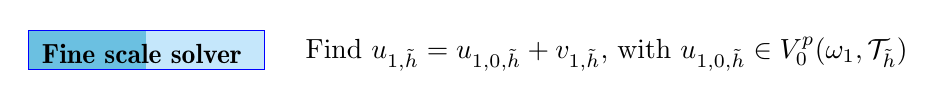
\begin{tikzpicture}
 	\filldraw [cyan!60!white!90!black](1.5, 0.5)--(0,0.5)--(0,0)--(1.5,0);
 	\draw [blue] (1.5, 0.5)--(0,0.5)--(0,0)--(1.5,0);
 	\filldraw [rr](1.5, 0)--(3,0)--(3,.5)--(1.5,0.5);
 	\draw [blue] (1.5, 0)--(3,0)--(3,0.5)--(1.5,0.5); 
 	\draw(0.05,0.2) node[right] {\textbf{Fine scale solver}};
 	\draw(3.4, 0.2)node[right] {Find $\uhone=\uhonezero + \vhone$, with $\uhonezero\in V^p_0(\omega_1, \Thtilde)$};
 	\end{tikzpicture}

 such that 
\[ B_{1}(\uhonezero, \whtilde):=\int_{\omega_1}a \nabla \uhonezero \cdot\nabla \whtilde \d x=\int_{\omega_1}f \whtilde\d x, \cinq \forall \whtilde \in V^p_0(\omega_1, \Thtilde).\]

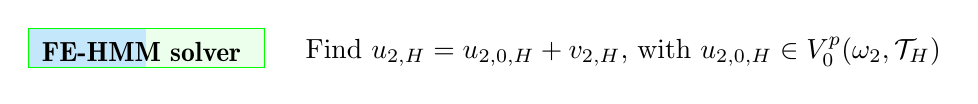
\begin{tikzpicture}
\filldraw [rr](1.5, 0.5)--(0,0.5)--(0,0)--(1.5,0);
\draw [green] (1.5, 0.5)--(0,0.5)--(0,0)--(1.5,0);
\filldraw [gr!60](1.5, 0)--(3,0)--(3,.5)--(1.5,0.5);
\draw [green] (1.5, 0)--(3,0)--(3,0.5)--(1.5,0.5); 
\draw(0.05,0.2) node[right] {\textbf{FE-HMM solver}};
\draw(3.4, 0.2)node[right] {Find $\uhtwo=\uhtwozero + \vhtwo$, with $\uhtwozero\in V^p_{0}(\omega_2, \TH)$};
\end{tikzpicture}

such that, $\forall w_H\in V^p_0(\omega_2, \TH)$ \[
 B_{2}(\uhtwozero, w_{H}):=\hspace{-0.2cm} \sum_{K\in \TH} \sum_{j=1}^J \frac{w_{j,K}}{|\Kdj|}\int_{\Kdj}\hspace{-0.2cm}a\nabla u^h_j \cdot\nabla w^h_j\d x=\int_{\omega_2}\hspace{-0.2cm}f^0w_H \d x,
 \]where $u^h_j,w^h_j$ are solutions of a micro problem involving the tensor $a$ on $\Kdj$. The solution ($\vhone$, $\vhtwo$) is the critical point of
 \begin{align*}
 \mathcal{L}(\vhone, \lhone, \vhtwo, \lhtwo)&=\frac{1}{2}\normL{(\uhonezero+ \vhone)-(\uhtwozero+ \vhtwo)}{2}{\omega_0}^2 \\
 &- B_1(\vhone, \lhone)- B_{2}(\vhtwo, \lhtwo).
 \end{align*}
 }


%%%%%%%%%%%%%%%%%%%%%%%%%%%%%%%%%%%%%%%%%%%%%%%%%%%%%%%%%%%%%%%%%%%%%%%%%%%%%%%
\headerbox{Algorithm}{name=algo,column=1,row=0,below=FEobc}{
$\bullet$ \text{ Find } $\uonezero^{\htilde} \in  V^p_0(\omega_1, \Thtilde)$: $B_{1}^ {\htilde}(\uonezero^{\htilde}, w^{\htilde})= \int_{\omega_1}f w^{\htilde}\d x$, $\forall w^{\htilde} \in V^p_0(\omega_1, \Thtilde)$.
$\bullet$ \text{ Find } $\utwozero^{H} \in  V^p_0(\omega_2, \TH)$: $B_{2}^ {H}(\utwozero^{H}, w^{\htilde})= \int_{\omega_1}f w^{\htilde}\d x$, $\forall w^{\htilde} \in V^p_0(\omega_1, \Thtilde)$.
$\bullet$ \text{ Find } $\uonezero^{\htilde} \in  V^p_0(\omega_1, \Thtilde)$: $B_{1}^ {\htilde}(\uonezero^{\htilde}, w^{\htilde})= \int_{\omega_1}f w^{\htilde}\d x$, $\forall w^{\htilde} \in V^p_0(\omega_1, \Thtilde)$.
}
 %%%%%%%%%%%%%%%%%%%%%%%%%%%%%%%%%%%%%%%%%%%%%%%%%%%%%%%%%%%%%%%%%%%%%%%%%%%%%%
   \headerbox{A Priori Error Estimates}{name=apriori,column=1,row=0,below=algo}{
 %%%%%%%%%%%%%%%%%%%%%%%%%%%%%%%%%%%%%%%%%%%%%%%%%%%%%%%%%%%%%%%%%%%%%%%%%%%%%%
 \textbf{Fill here}
}
 

   \headerbox{References}{name=references,column=1,span=1,below=apriori}{

    \bibliographystyle{plain}
 \renewcommand{\section}[2]{\vskip 0.05em}
%  \begin{thebibliography}{3}
%
% \end{thebibliography}
\begin{thebibliography}{1}
	
	\bibitem{CGS16}
	Conrad, P. R. et al.
	\newblock Statistical analysis of differential equations: introducing probability measures on numerical solutions.
	\newblock {\em Stat. Comput.}, 2016.
	
	\bibitem{KaS2005}
	J. Kaipio and E. Somersalo.
	\newblock Statistical and Computational Inverse Problems.
	\newblock {\em Applied Mathematical Sciences}, 2005.
	
	\bibitem{Vih2012}
	M. Vihola.
	\newblock Robust adaptive Metropolis algorithm with coerced acceptance rate.
	\newblock {\em Stat. Comput.}, 2012.
		
\end{thebibliography}



 %%%%%%%%%%%%%%%%%%%%%%%%%%%%%%%%%%%%%%%%%%%%%%%%%%%%%%%%%%%%%%%%%%%%%%%%%%%%%%
   }


\end{poster}%
%
\end{document}
